\documentclass[1p,12pt]{elsarticle}

%% Paquetes del template base
\usepackage{amssymb}
\usepackage{lineno}
\usepackage{epsfig}
\usepackage[spanish]{babel}
\usepackage[labelsep=endash]{caption}

%% Paquetes adicionales necesarios para el contenido
\usepackage{graphicx}
\usepackage{amsmath}
\usepackage{booktabs}
\usepackage{array}
\usepackage{float}
\usepackage{multirow}
\usepackage{subfig}
\usepackage{enumitem}
\usepackage{xcolor}
\usepackage{listings}
\usepackage{hyperref}

%% Listings (bloques de arquitectura)
\definecolor{grisClaro}{RGB}{245,245,245}
\lstset{
  basicstyle=\ttfamily\small,
  backgroundcolor=\color{grisClaro},
  frame=single,
  breaklines=true,
  columns=fullflexible,
  keepspaces=true
}

\journal{Cátedra de Inteligencia Artificial}

\renewcommand{\figurename}{Fig.}
\renewcommand{\tablename}{Tab.}

%% Definición de comandos custom del template de la cátedra
%% (no forman parte del elsarticle estándar)
\newcommand{\autor}[1]{\author{#1}}
\newcommand{\catedra}[1]{\address{#1}}

%% ─────────────────────────────────────────────────────────────────────────────
\begin{document}

\begin{frontmatter}

\title{Detección automática de neumonía en radiografías de tórax mediante redes neuronales convolucionales}

\autor{Romano L.E., Ibañez M.A., Haurigot Posse O., Rodríguez N.M.}

\catedra{Cátedra de Inteligencia Artificial, Ingeniería en Sistemas de Información}

\begin{abstract}
\textbf{i) Problema.} La neumonía es una de las principales causas de mortalidad infantil según la OMS, y su diagnóstico a partir de radiografías de tórax requiere un radiólogo entrenado del que muchas regiones carecen. El problema presenta un desbalance marcado entre clases y exige balancear sensibilidad con especificidad.

\textbf{ii) Método, técnica y herramientas.} Se trabajó con el dataset \textit{Chest X-Ray Images (Pneumonia)} de Kermany et al.\ \cite{kermany2018} (5\,248 imágenes, desbalance 1:3). Se entrenaron y compararon tres arquitecturas: \textbf{VGG16} \cite{simonyan2014} (15,11\,M parámetros) y \textbf{ResNet50} \cite{he2015} (24,77\,M parámetros), ambos con Transfer Learning en dos fases; y \textbf{PneuNet} \cite{saranyaraj2025} (154\,K parámetros), red liviana con bloques SE \cite{hu2018}, ASPP \cite{chen2017} y \textit{learnable pooling}, entrenada desde cero. El preprocesamiento incluyó \textit{data augmentation} y \textit{class weights} para mitigar el desbalance. Entorno: TensorFlow 2.21 + Keras 3.

\textbf{iii) Resultado principal y conclusión.} Los tres modelos superan el 89\,\% de \textit{accuracy} y el 96\,\% de AUC-ROC. \textbf{VGG16} lidera en F1 (97,09\,\%), Recall (98,46\,\%) y AUC (99,24\,\%). \textbf{ResNet50} destaca en Precisión (98,08\,\%) y Especificidad (97,01\,\%). \textbf{PneuNet}, 98$\times$ más pequeño, alcanza F1\,=\,91,13\,\% pero pierde 56 de las 390 neumonías del test (Recall\,=\,85,64\,\%). La elección depende del contexto: máxima calidad diagnóstica (VGG16), menor tasa de falsos positivos (ResNet50) o restricciones de hardware (PneuNet).
\end{abstract}

\begin{keyword}
redes neuronales convolucionales \sep transfer learning \sep fine-tuning \sep VGG16 \sep ResNet50 \sep depthwise separable convolutions \sep SE block \sep ASPP \sep clasificación de imágenes médicas \sep AUC-ROC
\end{keyword}

\end{frontmatter}

%% ─────────────────────────────────────────────────────────────────────────────
\section{Introducción}
\label{sec:intro}

La inteligencia artificial aplicada a imágenes médicas tiene impacto directo en la práctica clínica. La detección automática de neumonía en radiografías de tórax es un \textit{benchmark} clásico: clasificación binaria con datos accesibles, frontera sutil entre clases y costo elevado del falso negativo.

La cátedra de Inteligencia Artificial propuso el siguiente marco para el TP3: (1) elegir un dataset de la lista publicada; (2) tomar dos modelos de \texttt{keras.applications} y un tercer modelo surgido de un \textit{paper} sobre la temática; (3) aplicar Transfer Learning cuando se considere necesario y justificar las decisiones; (4) entregar un informe y defender el trabajo.

El grupo eligió el dataset \textit{Chest X-Ray} de Kermany et al.\ \cite{kermany2018} por su relevancia clínica, tamaño manejable ($\approx$5\,K imágenes) y desbalance marcado que plantea un problema realista y formativo. Los modelos seleccionados fueron \textbf{VGG16} \cite{simonyan2014} y \textbf{ResNet50} \cite{he2015} como los dos modelos de Keras Applications, y \textbf{PneuNet} \cite{saranyaraj2025} como modelo del \textit{paper}: una red liviana para radiografías con 154\,K parámetros.

%% ─────────────────────────────────────────────────────────────────────────────
\section{Marco teórico}
\label{sec:marco}

\subsection{Redes neuronales convolucionales (CNN)}

Una CNN aplica filtros aprendibles a la imagen de entrada, produciendo \textit{feature maps} que resaltan patrones locales. El convolucionado 2D se define como:
\begin{equation}
  S(i,j) = (K * I)(i,j) = \sum_m \sum_n I(i+m,\, j+n)\, K(m,n)
  \label{eq:conv}
\end{equation}
La red cierra con una neurona de salida con activación \textbf{sigmoide} $\hat{p} = \sigma(z) = (1+e^{-z})^{-1}$, que da la probabilidad de que la radiografía corresponda a neumonía.

\subsection{Backpropagation y vanishing gradient}

El entrenamiento minimiza la \textit{binary cross-entropy}:
\begin{equation}
  \mathcal{L}(y, \hat{p}) = -\bigl[y \log \hat{p} + (1-y) \log (1-\hat{p})\bigr]
  \label{eq:bce}
\end{equation}
mediante el optimizador Adam \cite{kingma2014} y retropropagación del gradiente capa por capa \cite{rumelhart1986}. En redes muy profundas el gradiente se atenúa progresivamente (\textit{vanishing gradient}), dificultando el aprendizaje en capas tempranas.

\subsection{Transfer Learning}

El Transfer Learning aprovecha pesos pre-entrenados en \textit{ImageNet} (1,2\,M imágenes, 1000 clases) en lugar de entrenar desde cero con pocos datos. Se aplicó un esquema de \textbf{dos fases}: (1) \textit{feature extraction} con la base congelada y LR\,=\,$10^{-3}$; (2) \textit{fine-tuning} de las últimas capas de la base con LR\,=\,$10^{-5}$ para evitar \textit{catastrophic forgetting}.

\subsection{VGG16}

VGG16 \cite{simonyan2014} tiene 16 capas con pesos (13 conv + 3 dense), bloques uniformes \texttt{conv~3$\times$3 $\to$ conv~3$\times$3 $\to$ max-pool} y $\approx$138\,M de parámetros originales. En este TP se usa con \texttt{include\_top=False} y una cabeza nueva (15,11\,M de parámetros totales).

\subsection{ResNet50 y conexiones residuales}

ResNet50 \cite{he2015} resuelve el \textit{vanishing gradient} con \textbf{skip connections}: cada bloque aprende el residuo $F(x) = H(x) - x$ y devuelve $F(x) + x$, creando un atajo por el que el gradiente fluye sin degradarse. Tiene 24,77\,M de parámetros totales en nuestra configuración.

\subsection{PneuNet y mecanismos modernos}

PneuNet \cite{saranyaraj2025} es una red liviana de 154\,K parámetros con cuatro mecanismos:
\begin{itemize}[noitemsep]
  \item \textbf{Depthwise Separable Convolutions:} descomponen una convolución estándar en \textit{depthwise} + \textit{pointwise} (1$\times$1), reduciendo el costo $\approx$8$\times$.
  \item \textbf{Bloque SE} \cite{hu2018}: aprende la importancia relativa de cada canal y reescala los \textit{feature maps} en consecuencia.
  \item \textbf{ASPP} \cite{chen2017}: aplica convoluciones dilatadas en paralelo para capturar contexto a múltiples escalas; clave cuando las lesiones tienen tamaños variables.
  \item \textbf{Learnable Pooling:} genera un mapa de atención espacial para ignorar el fondo negro de las radiografías y enfocarse en los pulmones.
\end{itemize}

\subsection{Métricas de evaluación}

A partir de los conteos básicos (TP, TN, FP, FN) se derivan las métricas del TP (Tab.~\ref{tab:metricas_def}).

\begin{table}[h]
\centering
\caption{Métricas de evaluación utilizadas.}
\label{tab:metricas_def}
\begin{tabular}{lll}
\hline
\textbf{Métrica} & \textbf{Fórmula} & \textbf{Interpretación} \\
\hline
Accuracy       & $(TP+TN)/(TP+TN+FP+FN)$ & Proporción de aciertos \\
Precision      & $TP/(TP+FP)$             & Costo del falso positivo \\
Recall         & $TP/(TP+FN)$             & Crítica en diagnóstico médico \\
F1-Score       & $2PR/(P+R)$              & Balance Precision-Recall \\
Especificidad  & $TN/(TN+FP)$             & Complementa al Recall \\
AUC-ROC        & Área bajo curva ROC      & Discriminación a todos los umbrales \\
\hline
\end{tabular}
\end{table}

En diagnóstico médico, el \textbf{Recall} (sensibilidad) suele ser la métrica más crítica: un falso negativo implica dejar a un paciente enfermo sin diagnosticar.

%% ─────────────────────────────────────────────────────────────────────────────
\section{Propuesta de desarrollo}
\label{sec:propuesta}

\subsection{Dataset}

Se trabajó con el dataset \textbf{Chest X-Ray Images (Pneumonia)} de Kermany et al.\ \cite{kermany2018}, disponible en Kaggle. La distribución se muestra en Tab.~\ref{tab:dataset}.

\begin{table}[h]
\centering
\caption{Distribución del dataset.}
\label{tab:dataset}
\begin{tabular}{lrrr}
\hline
\textbf{Split} & \textbf{NORMAL} & \textbf{PNEUMONIA} & \textbf{Total} \\
\hline
Train (original)    & 1\,349 & 3\,883 & 5\,232 \\
Train (80\,\%)      & \multicolumn{2}{c}{--} & 4\,187 \\
Validación (20\,\%) & \multicolumn{2}{c}{--} & 1\,045 \\
Test                & 234 & 390 & 624 \\
\hline
\end{tabular}
\end{table}

El desbalance \textbf{1:3} a favor de PNEUMONIA es problemático: un clasificador trivial que siempre predijera ``neumonía'' obtendría 62,5\,\% de \textit{accuracy} sin aprender nada. Para mitigarlo se aplicaron \textit{class weights} ($w_i = n_{total}/(n_{clases} \cdot n_i)$: NORMAL $\to$ 1,94; PNEUMONIA $\to$ 0,67) y validación estratificada con \texttt{validation\_split=0.2}.

\begin{figure}[h]
\centering
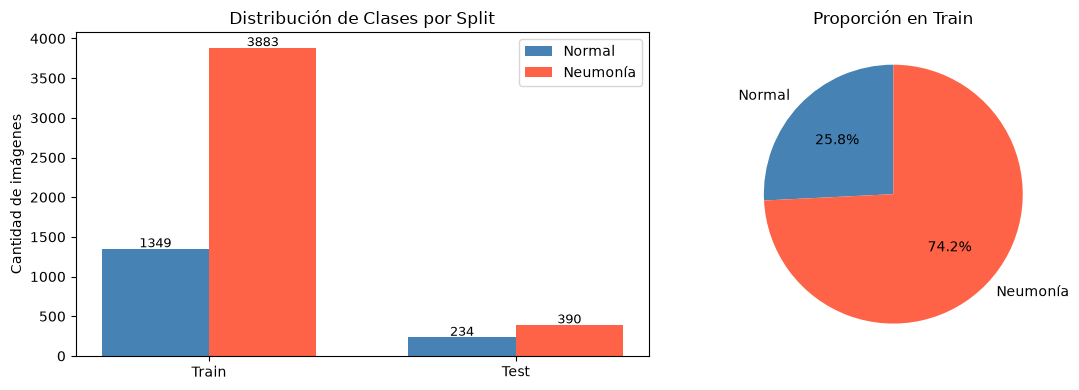
\includegraphics[width=0.85\linewidth]{figures/dataset_distribucion.png}
\caption{Distribución de clases por split (barras) y proporción en train (torta).}
\label{fig:distribucion}
\end{figure}

\begin{figure}[h]
\centering
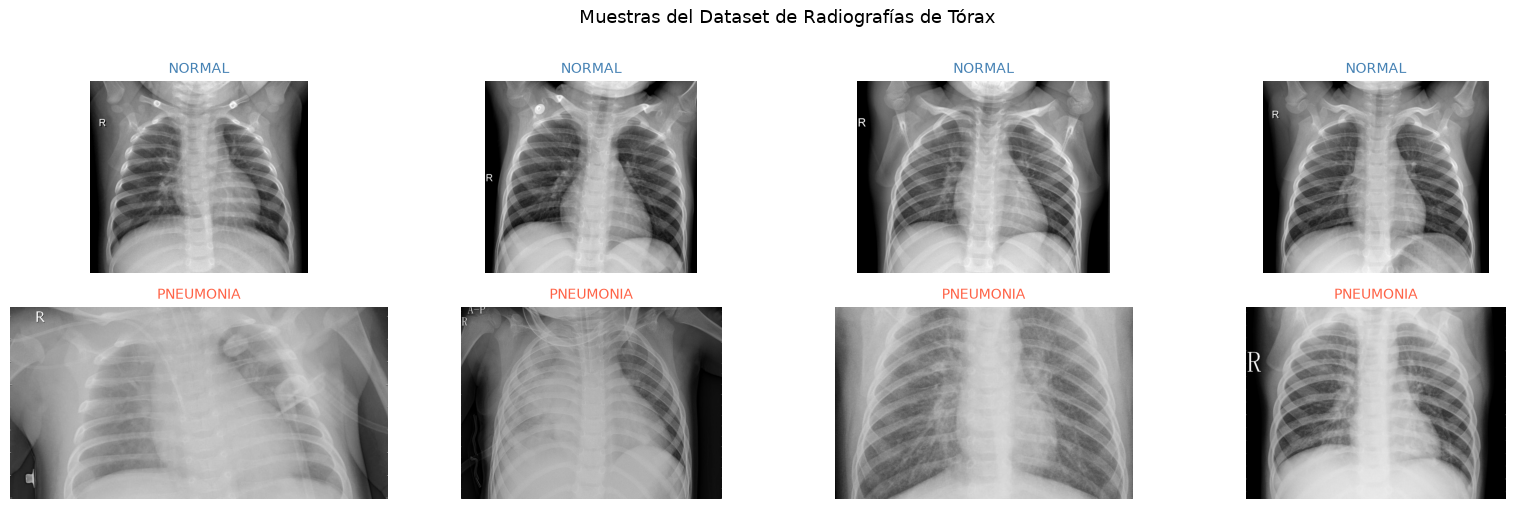
\includegraphics[width=0.85\linewidth]{figures/dataset_muestra.png}
\caption{Muestra del dataset: fila superior NORMAL, inferior PNEUMONIA.}
\label{fig:muestra}
\end{figure}

\subsection{Preprocesamiento y data augmentation}

Para VGG16 y ResNet50 se aplicó \texttt{preprocess\_input} específico de cada arquitectura (normalización según estadísticas de \textit{ImageNet}). Para PneuNet, normalización simple $\hat{x} = x/255$. El generador de entrenamiento aplicó \textit{data augmentation in-memory}: rotación $\pm$10°, zoom 10\,\%, \textit{flip horizontal}, desplazamientos 5\,\% y variación de brillo $\pm$10\,\%. La augmentación se aplicó \textbf{solo al entrenamiento}; validación y test se evaluaron con imágenes originales.

\subsection{Arquitectura A — VGG16 con Transfer Learning en dos fases}

\textbf{Fase 1 (Transfer Learning):} base VGG16 congelada. Cabeza nueva:

\begin{lstlisting}
Input(224x224x3)
+-- VGG16 (congelada)          -> (None, 7, 7, 512)
    +-- GlobalAveragePooling2D -> (None, 512)
        +-- Dense(512, ReLU) -> BatchNorm -> Dropout(0.5)
            +-- Dense(256, ReLU) -> Dropout(0.3)
                +-- Dense(1, Sigmoid)    -> p_hat
\end{lstlisting}

Adam, LR\,=\,$10^{-3}$, hasta 15 épocas, con \texttt{EarlyStopping(patience=4)}, \texttt{ModelCheckpoint} y \texttt{ReduceLROnPlateau}.

\textbf{Fase 2 (Fine-Tuning):} se descongelaron las últimas 4 capas de la base y se re-compiló con LR\,=\,$10^{-5}$ (100$\times$ menor) para evitar \textit{catastrophic forgetting}. Hasta 10 épocas, \texttt{EarlyStopping(patience=5)}.

\subsection{Arquitectura B — ResNet50 con Transfer Learning en dos fases}

Misma cabeza que VGG16, montada sobre \texttt{ResNet50(weights='imagenet', include\_top=False)}. En el fine-tuning se descongelaron las \textbf{últimas 10 capas} (más que en VGG16) porque las \textit{skip connections} estabilizan el gradiente y reducen el riesgo de degradar las representaciones.

\subsection{Arquitectura C — PneuNet (entrenada desde cero)}

\begin{lstlisting}
Input(224x224x3)
+-- Stem + 4 ramas paralelas (Conv 3x3 + 3x DSep, cada una Dropout 0.3)
    -> Concatenar (128 canales)
    -> SE Block (ratio 16)
    -> Depthwise stride=2 (downsampling)
    -> ASPP (dilataciones 1x1, 3x3 d=1, 3x3 d=3, 3x3 d=6)
    -> Learnable Pooling -> Dropout(0.3)
    -> Dense(1, Sigmoid) -> p_hat
\end{lstlisting}

Adam, LR\,=\,$10^{-3}$, hasta 50 épocas, \texttt{EarlyStopping(patience=7)}, regularización L2 y \textit{class weights}. PneuNet no usa Transfer Learning: con 154\,K parámetros y $\approx$4\,K imágenes es viable entrenar desde cero sin \textit{overfitting} severo, eliminando la dependencia de pesos externos ($>$100\,MB).

%% ─────────────────────────────────────────────────────────────────────────────
\section{Experimentos y resultados}
\label{sec:resultados}

\subsection{Curvas de entrenamiento}

Las curvas de VGG16 y ResNet50 (Fig.~\ref{fig:train_curves}) muestran que la fase de Transfer Learning ya alcanza \textit{accuracy} de validación $>$95\,\% en pocas épocas. El fine-tuning (marcado con línea punteada en la época 11) aporta mejoras adicionales modestas pero consistentes. PneuNet muestra mayor variabilidad inicial al aprender todo desde cero, convergiendo con apoyo de \texttt{EarlyStopping}.

\begin{figure}[h]
\centering
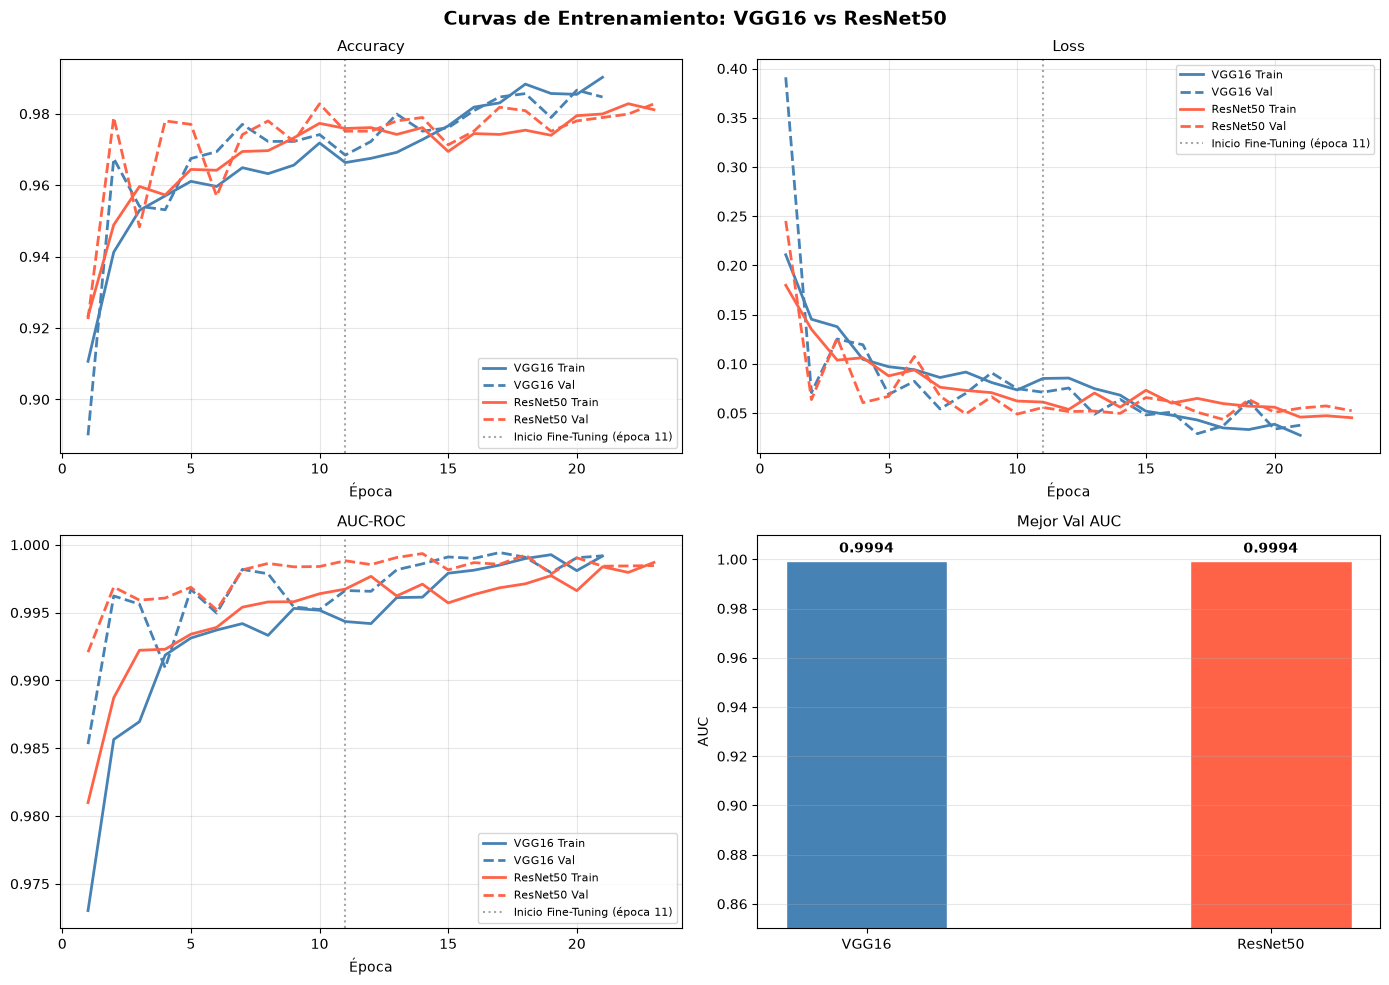
\includegraphics[width=\linewidth]{figures/train_curves_vgg_resnet.png}
\caption{Curvas de entrenamiento de VGG16 y ResNet50. La línea punteada marca el inicio del fine-tuning (época 11).}
\label{fig:train_curves}
\end{figure}

\subsection{Matrices de confusión}

Las matrices de confusión del \textit{test set} (624 imágenes) se muestran en las Fig.~\ref{fig:confusion2} y \ref{fig:confusion3}. La Tab.~\ref{tab:errores} resume los errores por modelo.

\begin{figure}[h]
\centering
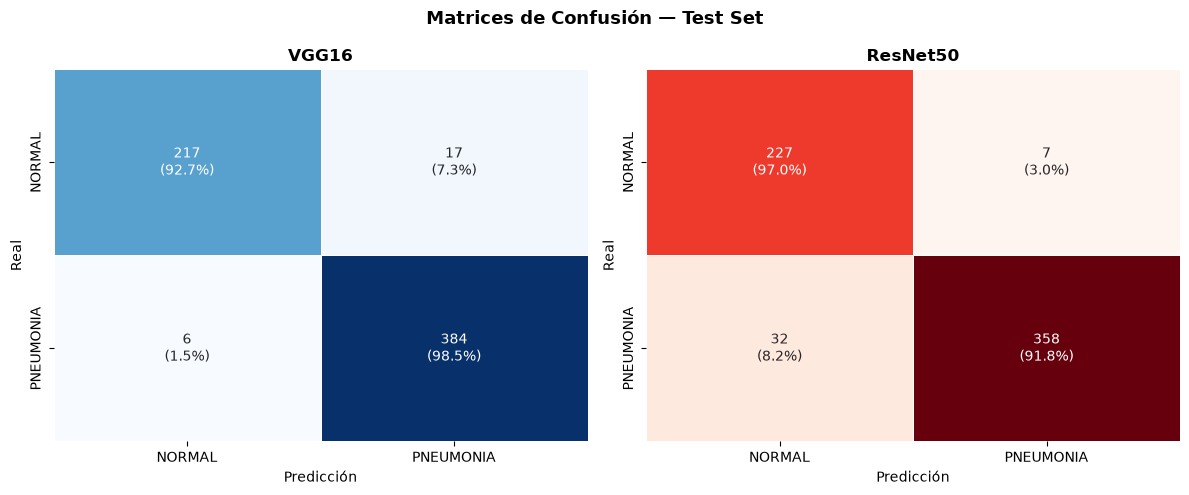
\includegraphics[width=0.85\linewidth]{figures/confusion_vgg_resnet.png}
\caption{Matrices de confusión de VGG16 y ResNet50.}
\label{fig:confusion2}
\end{figure}

\begin{figure}[h]
\centering
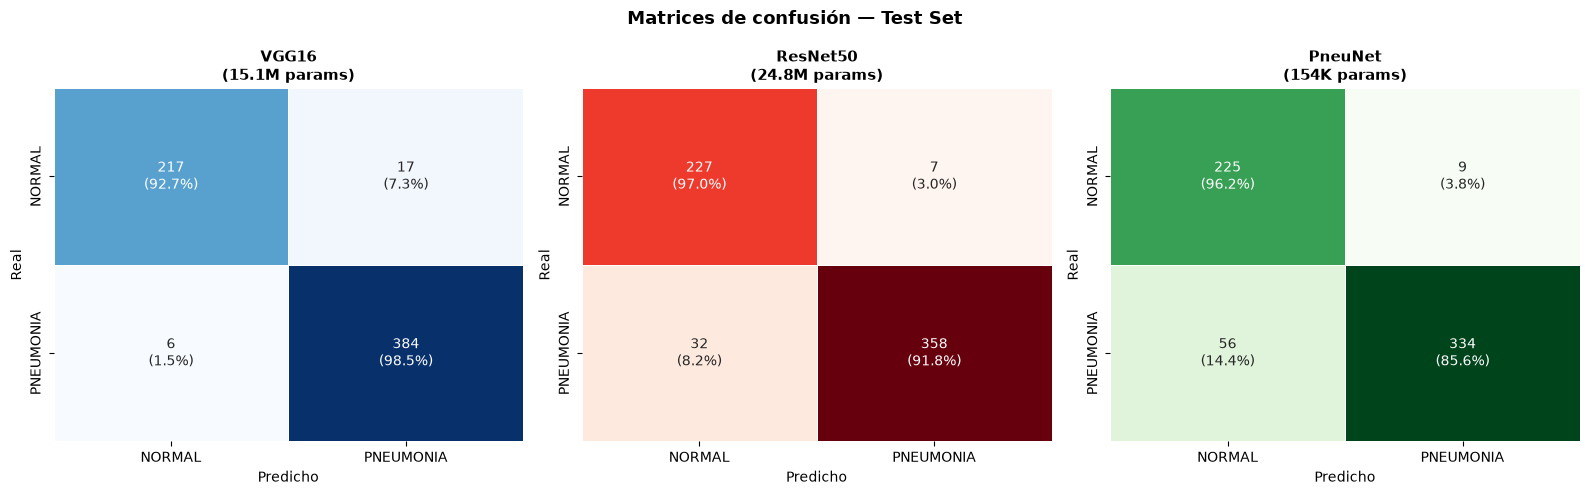
\includegraphics[width=\linewidth]{figures/confusion_3modelos.png}
\caption{Matrices de confusión de los tres modelos.}
\label{fig:confusion3}
\end{figure}

\begin{table}[h]
\centering
\caption{Resumen de errores por modelo (test set, 624 imágenes).}
\label{tab:errores}
\begin{tabular}{lrrrrrr}
\hline
\textbf{Modelo} & \textbf{TP} & \textbf{FP} & \textbf{FN} & \textbf{TN} & \textbf{Errores} & \textbf{Error principal} \\
\hline
VGG16    & 384 & 17 &  6 & 217 & 23 (3,7\,\%)  & Falsos positivos \\
ResNet50 & 358 &  7 & 32 & 227 & 39 (6,2\,\%)  & Falsos negativos \\
PneuNet  & 334 &  9 & 56 & 225 & 65 (10,4\,\%) & Falsos negativos \\
\hline
\end{tabular}
\end{table}

\subsection{Curvas ROC}

La Fig.~\ref{fig:roc} muestra las curvas ROC para los tres modelos. Los AUC-ROC son: VGG16\,=\,0,9924; ResNet50\,=\,0,9846; PneuNet\,=\,0,9699. Los tres se alejan claramente de la diagonal (clasificador aleatorio), confirmando que todos discriminan entre clases.

\begin{figure}[h]
\centering
\subfloat[VGG16 vs ResNet50.]{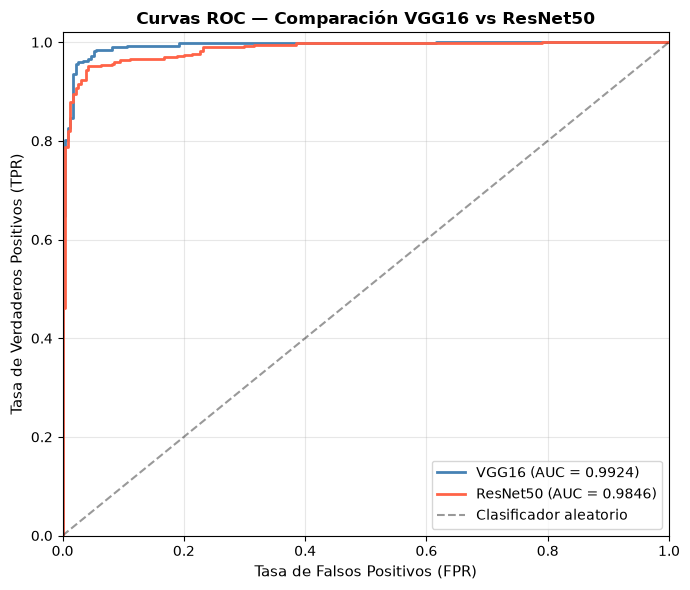
\includegraphics[width=0.48\linewidth]{figures/roc_vgg_resnet.png}}
\hfill
\subfloat[Los tres modelos.]{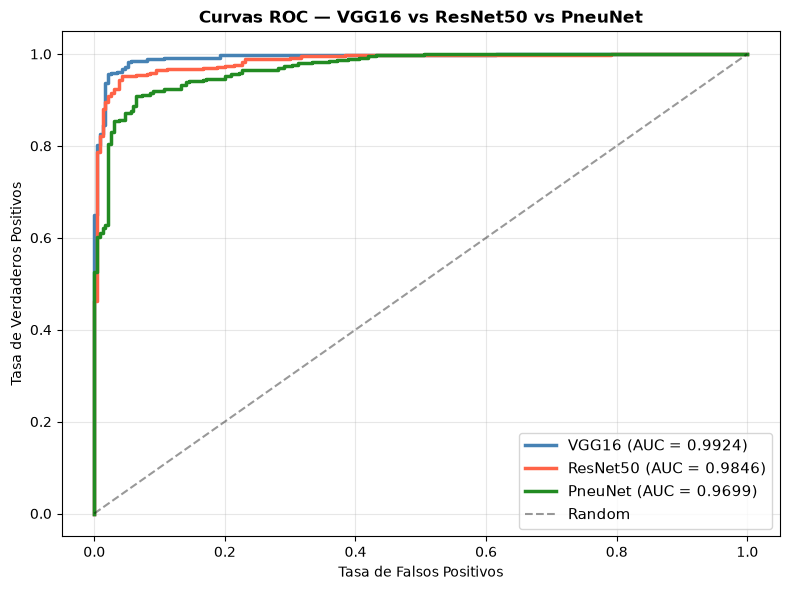
\includegraphics[width=0.48\linewidth]{figures/roc_3modelos.png}}
\caption{Curvas ROC en el test set. La diagonal representa un clasificador aleatorio (AUC\,=\,0,5).}
\label{fig:roc}
\end{figure}

\subsection{Comparación de métricas}

La Tab.~\ref{tab:metricas} resume las métricas en el test set con umbral 0,5, y la Fig.~\ref{fig:metricas} las visualiza.

\begin{table}[h]
\centering
\caption{Métricas comparativas en el test set (umbral 0,5). En negrita el mejor valor por columna.}
\label{tab:metricas}
\begin{tabular}{lrrrrrr}
\hline
\textbf{Modelo} & \textbf{Accuracy} & \textbf{Precision} & \textbf{Recall} & \textbf{F1} & \textbf{AUC} & \textbf{Espec.} \\
\hline
\textbf{VGG16}   & \textbf{96,31} & 95,76 & \textbf{98,46} & \textbf{97,09} & \textbf{99,24} & 92,74 \\
ResNet50         & 93,75 & \textbf{98,08} & 91,79 & 94,83 & 98,46 & \textbf{97,01} \\
PneuNet          & 89,58 & 97,38 & 85,64 & 91,13 & 96,99 & 96,15 \\
\hline
\end{tabular}
\end{table}

\begin{figure}[h]
\centering
\subfloat[VGG16 vs ResNet50.]{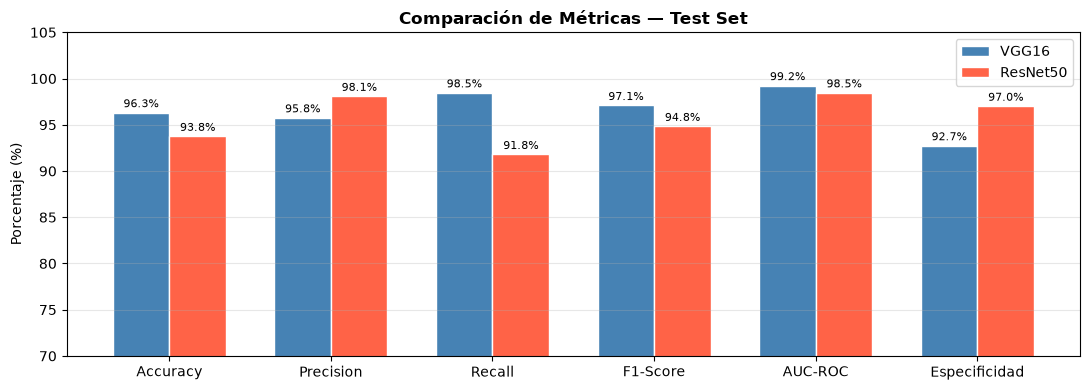
\includegraphics[width=0.48\linewidth]{figures/metricas_vgg_resnet.png}}
\hfill
\subfloat[Los tres modelos.]{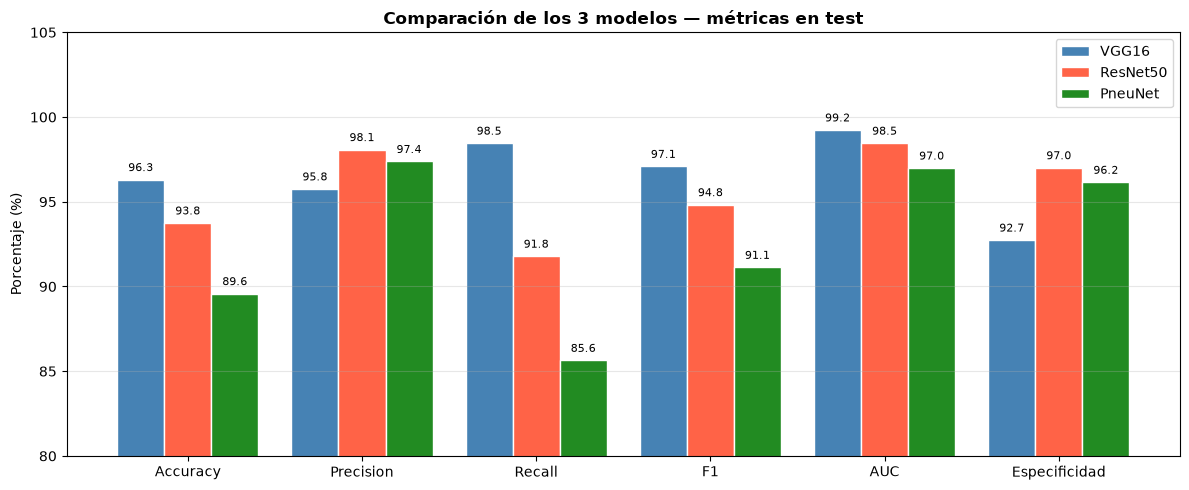
\includegraphics[width=0.48\linewidth]{figures/metricas_3modelos.png}}
\caption{Comparación visual de métricas en el test set.}
\label{fig:metricas}
\end{figure}

\subsection{Trade-off entre tamaño y rendimiento}

Los tres modelos tienen tamaños muy distintos (Tab.~\ref{tab:params}). Las Fig.~\ref{fig:params} muestran la diferencia de escala y el \textit{trade-off} accuracy--tamaño.

\begin{table}[h]
\centering
\caption{Comparación de parámetros.}
\label{tab:params}
\begin{tabular}{lrr}
\hline
\textbf{Modelo} & \textbf{Parámetros} & \textbf{Ratio vs PneuNet} \\
\hline
VGG16    & 15,11\,M &  98$\times$ \\
ResNet50 & 24,77\,M & 161$\times$ \\
PneuNet  & 154\,K   &   1$\times$ \\
\hline
\end{tabular}
\end{table}

\begin{figure}[h]
\centering
\subfloat[Comparación de tamaño (lineal y log).]{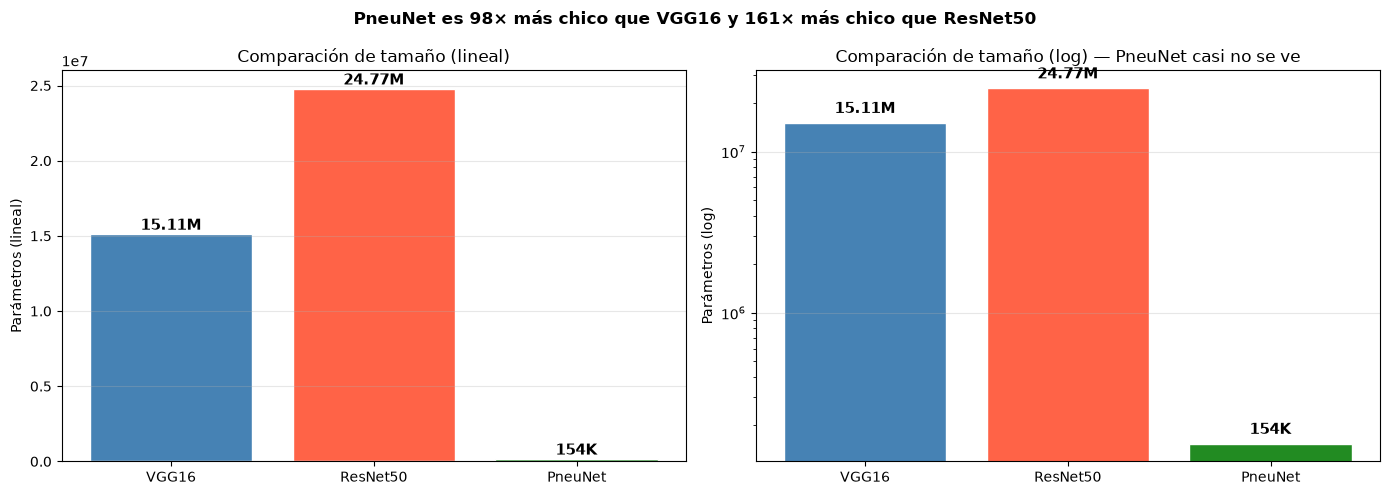
\includegraphics[width=0.48\linewidth]{figures/parametros_3modelos.png}}
\hfill
\subfloat[Accuracy vs parámetros (burbuja = Recall).]{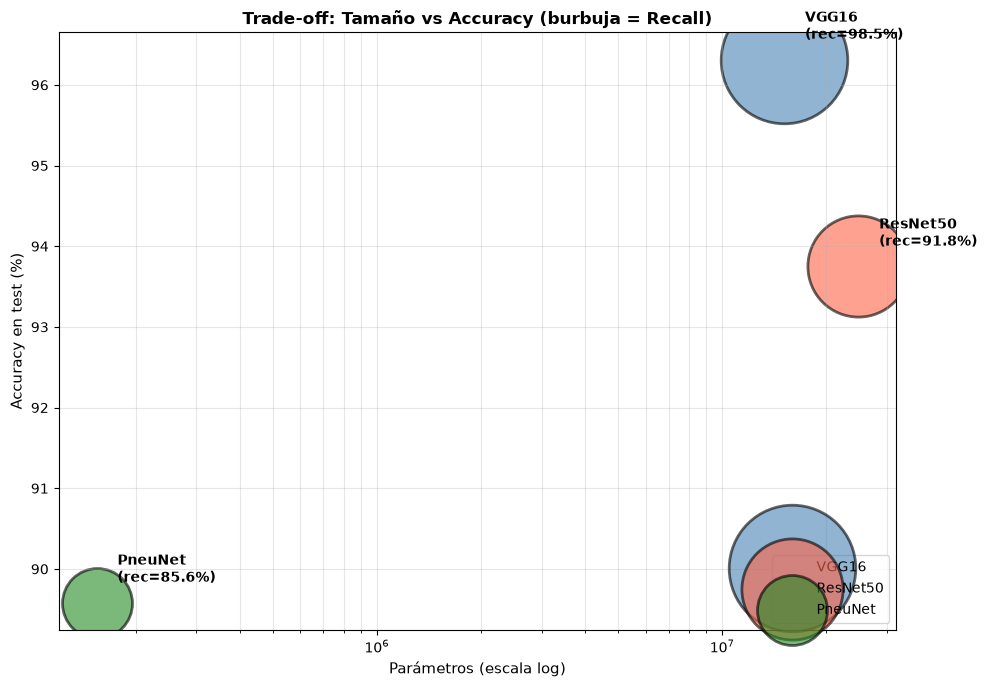
\includegraphics[width=0.48\linewidth]{figures/tradeoff_accuracy_params.png}}
\caption{Trade-off entre tamaño del modelo y rendimiento.}
\label{fig:params}
\end{figure}

\subsection{Análisis de falsos negativos}

En \textit{screening} médico, la pregunta más importante es cuántas neumonías no detectó cada modelo. La Fig.~\ref{fig:fn} y la Tab.~\ref{tab:fn} muestran los resultados.

\begin{figure}[h]
\centering
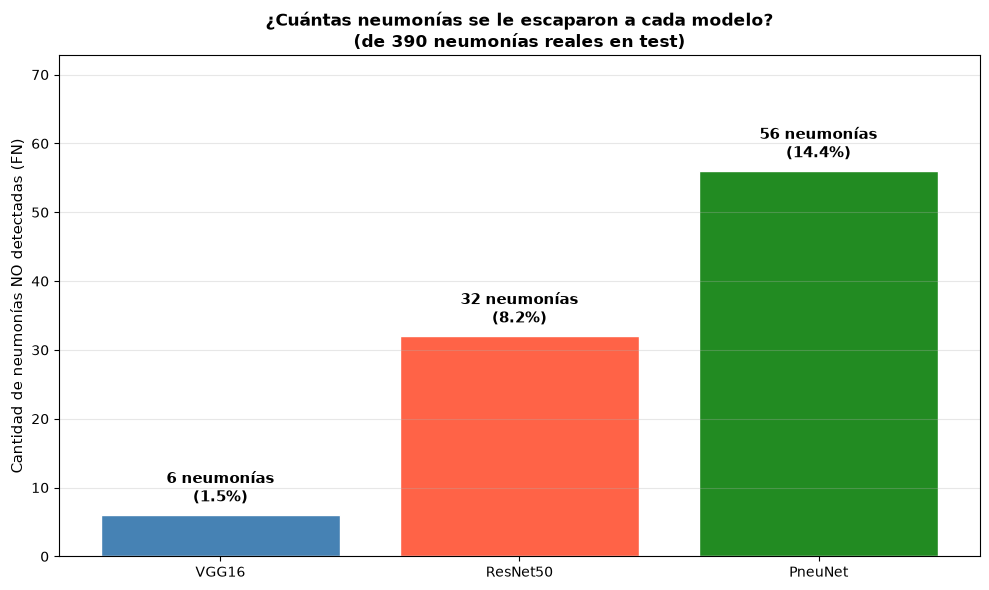
\includegraphics[width=0.65\linewidth]{figures/falsos_negativos.png}
\caption{Neumonías no detectadas (falsos negativos) por modelo, de 390 totales en test.}
\label{fig:fn}
\end{figure}

\begin{table}[h]
\centering
\caption{Falsos negativos por modelo.}
\label{tab:fn}
\begin{tabular}{lrr}
\hline
\textbf{Modelo} & \textbf{Neumonías no detectadas} & \textbf{Porcentaje} \\
\hline
VGG16    &  6 &  1,5\,\% \\
ResNet50 & 32 &  8,2\,\% \\
PneuNet  & 56 & 14,4\,\% \\
\hline
\end{tabular}
\end{table}

La diferencia entre PneuNet y VGG16 es de 50 neumonías no detectadas: ese es el costo concreto de ser 98$\times$ más pequeño.

\subsection{Análisis de errores cualitativo}

La Fig.~\ref{fig:errores} muestra muestras de imágenes mal clasificadas. La inspección cualitativa revela que los errores ocurren principalmente en: (a) neumonías leves con opacidades sutiles, (b) casos \textit{borderline} donde la frontera NORMAL/PNEUMONIA es difusa incluso para un radiólogo, y (c) radiografías con artefactos de pose u oclusión. Este patrón sugiere que el modelo es más confiable como \textbf{primer filtro} que como diagnóstico definitivo.

\begin{figure}[h]
\centering
\subfloat[VGG16 (23 errores).]{
\includegraphics[width=0.48\linewidth]{figures/errores_vgg16.png}}
\hfill
\subfloat[ResNet50 (39 errores).]{
\includegraphics[width=0.48\linewidth]{figures/errores_resnet50.png}}
\caption{Ejemplos mal clasificados por VGG16 y ResNet50.}
\label{fig:errores}
\end{figure}

\subsection{Análisis de overfitting}

La Fig.~\ref{fig:overfitting} compara la \textit{accuracy} de entrenamiento con la de test para las versiones TL y FT de VGG16 y ResNet50. Todas las brechas son menores al 2\,\%, validando que las técnicas de regularización (augmentación, \textit{class weights}, \textit{dropout}, \textit{early stopping}, \texttt{ReduceLROnPlateau}) controlaron el sobreajuste.

\begin{figure}[h]
\centering
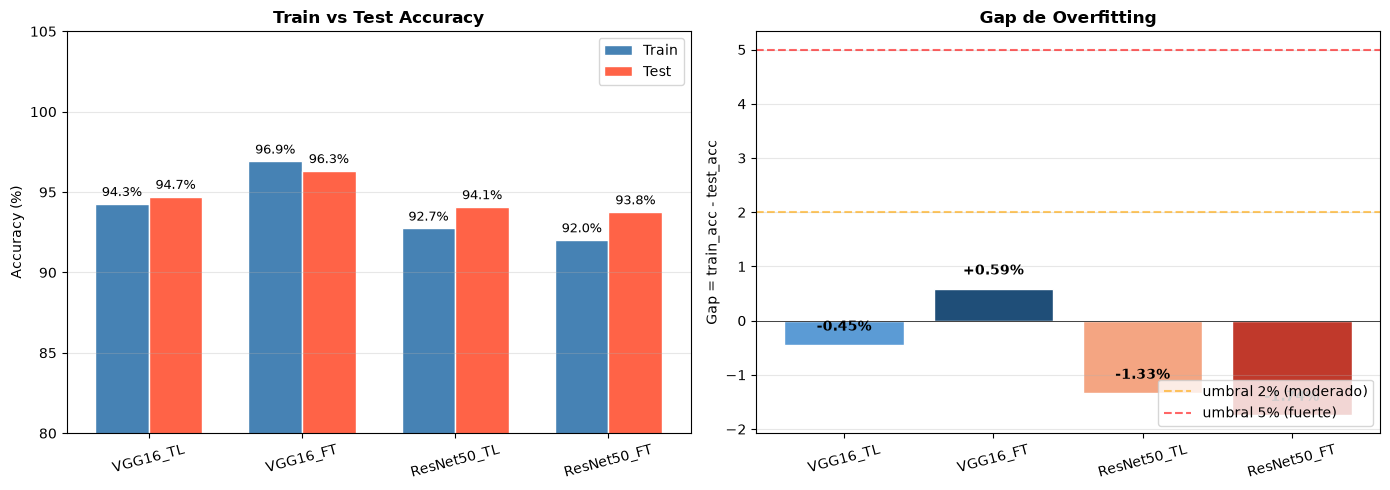
\includegraphics[width=\linewidth]{figures/overfitting_train_test.png}
\caption{Train vs test accuracy y gap de overfitting para los modelos TL y FT. Las brechas son menores al umbral moderado del 2\,\%.}
\label{fig:overfitting}
\end{figure}

\subsection{Variación del umbral de decisión}

La Fig.~\ref{fig:threshold} muestra el efecto de variar el umbral de decisión sobre las métricas. Bajar el umbral aumenta el Recall a costa de la Precisión. El umbral 0,5 es razonable, pero en producción puede calibrarse: por ejemplo, bajarlo a 0,3 en un sistema de \textit{screening} para maximizar la detección de casos positivos.

\begin{figure}[h]
\centering
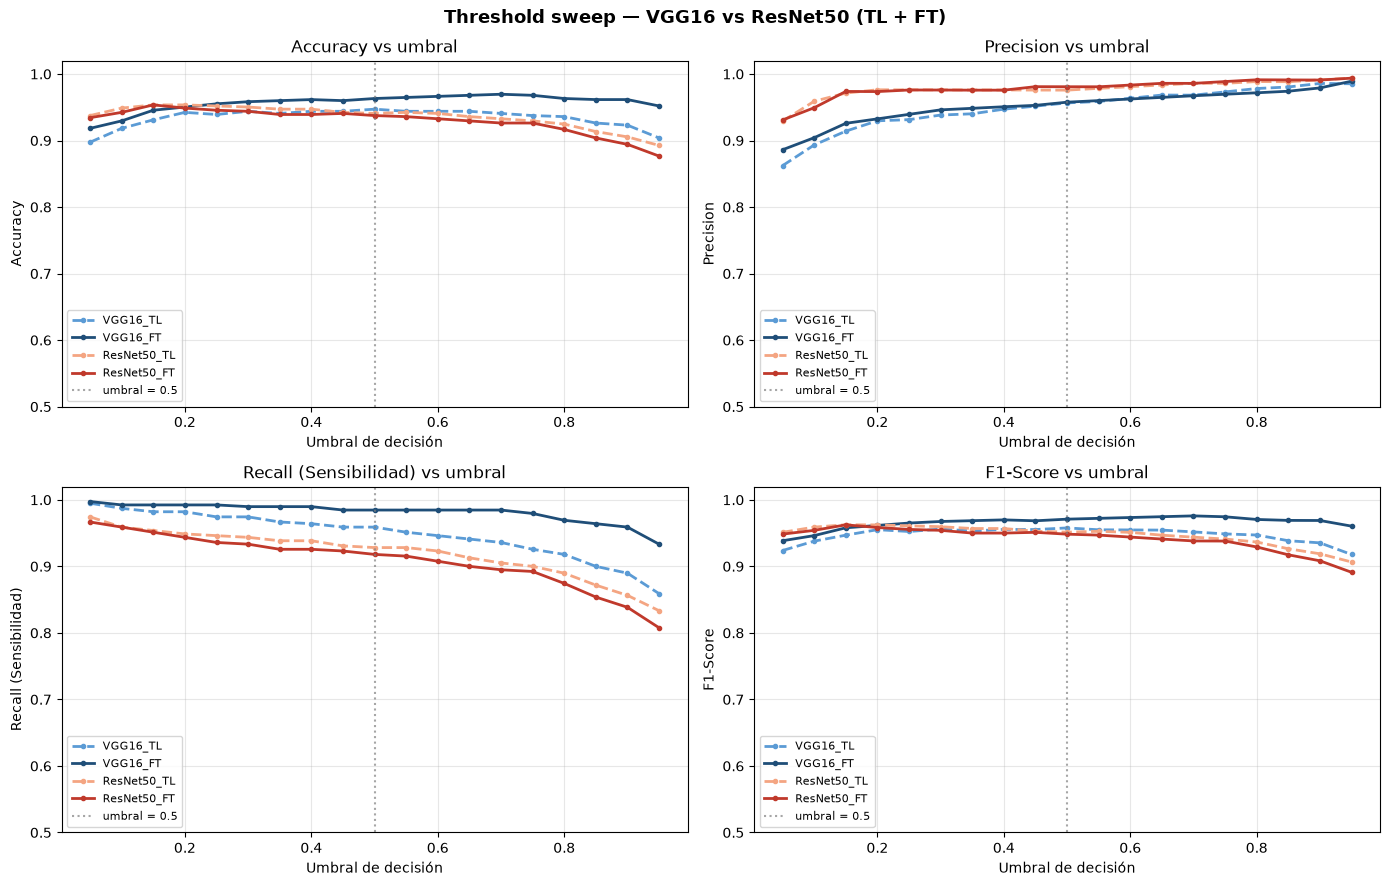
\includegraphics[width=\linewidth]{figures/threshold_sweep.png}
\caption{Threshold sweep: efecto del umbral en accuracy, precision, recall y F1 para VGG16 y ResNet50 (TL + FT).}
\label{fig:threshold}
\end{figure}

\subsection{Discusión}

\begin{enumerate}
  \item \textbf{El Transfer Learning con fine-tuning funciona.} VGG16 y ResNet50 alcanzan F1 $\geq$ 94,8\,\% sobre el test set, confirmando que las representaciones de bordes y texturas aprendidas en \textit{ImageNet} son transferibles a radiografías.
  \item \textbf{Las conexiones residuales no son decisivas con este dataset.} ResNet50 tiene menor accuracy y F1 que VGG16, aunque gana en Precisión y Especificidad. Con $\approx$4\,K imágenes, el modelo más grande sufre ligeramente más a pesar de la regularización.
  \item \textbf{PneuNet es competitivo pero no superior.} La diferencia de 12,8 puntos en Recall respecto a VGG16 pesa mucho en una aplicación médica.
  \item \textbf{El AUC-ROC de los tres modelos es $\geq$0,97.} Los casos \textit{borderline} son la principal fuente de errores.
\end{enumerate}

%% ─────────────────────────────────────────────────────────────────────────────
\section{Conclusiones}
\label{sec:conclusiones}

El trabajo cumplió todos los objetivos de la consigna. Los resultados muestran que \textbf{VGG16 con fine-tuning es la mejor opción} en términos de F1 (97,09\,\%), Recall (98,46\,\%) y AUC (99,24\,\%). \textbf{ResNet50} ofrece un balance diferente: mejor Precisión (98,08\,\%) y Especificidad (97,01\,\%), con un F1 algo menor (94,83\,\%). \textbf{PneuNet}, con 154\,K parámetros, alcanza Especificidad 96,15\,\% pero Recall 85,64\,\%, perdiendo 56 de las 390 neumonías del test.

Lecciones principales:
\begin{itemize}[noitemsep]
  \item El Transfer Learning es indispensable con pocos datos: sin él, entrenar VGG16 o ResNet50 sería prácticamente inviable.
  \item El desbalance de clases exige mitigación activa mediante \textit{class weights}.
  \item Métricas múltiples son indispensables: la \textit{accuracy} sola puede ser engañosa con clases desbalanceadas.
  \item No hay un ``mejor modelo'' absoluto: la elección depende del contexto, las restricciones de hardware y la tolerancia a cada tipo de error.
  \item La eficiencia y el rendimiento no siempre van de la mano: PneuNet logra 89,6\,\% de \textit{accuracy} con 98$\times$ menos parámetros, a un costo en Recall que debe evaluarse según la aplicación.
\end{itemize}

Como limitación, el dataset proviene de un único centro médico con imágenes pediátricas; generalizar a adultos o a otros centros requeriría re-entrenamiento.

%% ─────────────────────────────────────────────────────────────────────────────
\bibliographystyle{model1-num-names}
\bibliography{bibliografia}

\end{document}
